\section{Introduction}

	\subsection{The Standard Model of Particle Physics}

    Central to the moden study of particle physics is the standard model,
    \vspace{-1em}
    \begin{multline} \label{eqn:std-mod}
      L_{GWL} = \sum_{f} ( \bar{\Psi}_{f} ( i \gamma^\mu \partial \mu - m_{f} ) \Psi_{f} - eQ_{f} \bar{\Psi}_{f} \gamma^\mu \Psi_{f} A_{\mu} ) + \frac{g}{\sqrt{2}} \sum_{i} ( \bar{a}^i_L \gamma^\mu b^i_L W^+_\mu + \bar{b}^i_L \gamma^\mu a^i_L W^-_\mu )                        \\                           
              + \frac{g}{2x_w} \sum_f \bar{\Psi}_f \gamma^\mu ( I^3_f - 2s^2_w Q_f - I6e_f \gamma_5 ) \Psi_f Z_\mu - \frac{1}{4} | \partial_\mu A_v - \partial_v A_\mu - ie(W^-_\mu W^+_v - W^+_\mu W^-_v ) |^2                                         \\                                     
              - \frac{1}{2} | \partial_\mu W^+_v - \partial_v W^+_\mu - ie ( W^+_\mu A_v - W^+_v A_\mu ) + ig' c_w (W^+_\mu Z_v - W^+_v Z_\mu |^2 \\
              - \frac{1}{4} | \partial_\mu Z_v - \partial_v Z_\mu + ig' c_w (W^-_\mu W^+_v - W^+_\mu W^-_v ) |^2 - \frac{1}{2} M^2_\eta \eta^2  - \frac{gM^2_\eta}{8M_W} \eta^3  - \frac{g'^2 M^2_\eta}{32M_W}\eta^4    \\     
              + | M_W W^+_\mu + \frac{g}{2} \eta W^+_\mu |^2 + \frac{1}{2} | \partial_\mu \eta + i M_Z Z_\mu + \frac{ig}{2c_w} \eta Z_\mu |^2 - \sum_f \frac{g m_f}{2 M_W} \bar{\Psi}_f \Psi_f \eta.                                                                                
      \vspace{-1em}
    \end{multline}
    \vspace{-1em}

    The standard model, shown in equation \ref{eqn:std-mod}, is a quantum field theory that discribes the fundermental particles and how they interact.
    While this report does not require, or attempt, a detailed understanding the intricate detail of the stardard model;
    the aim of many particle physics experiments is to varify, measure and expand the model.
    Dispite being the current best theory to explain particle interactions, the model is not complete.
    There are many undescribed phemomina, such as the matter domination in the universe, that require physics behond the standard model in order to be described.
    To that end, major international efforts, namely in the form of the Large Hardron Collider, aim to gain further knowledge and understanding of the underlying physics of the universe. \cite{ref:std}

  % \subsection{Field Programable Gate Arrays}

  \subsection{The LHCb Experiment}

    One experiment at the Large Hadrom Colider is Large Hadron Colider beauty (LHCb).
    Located at intersection point 8, LHCb is designed to study rare particly physics phemonena, such as lepton flavour violation and CP violation. 
    The decays studied in the LCHb are via exotic hadronic decays of Bottom or Charm quarks that form sort lived hardons. 
    These hardons, commonly B mesons, travel in the order of mm's in the detector before decaying. 
    As such, B meson decays can be identied by decay products that propogate via a secondary vertex.

    \begin{figure}[h!]
      \centering
      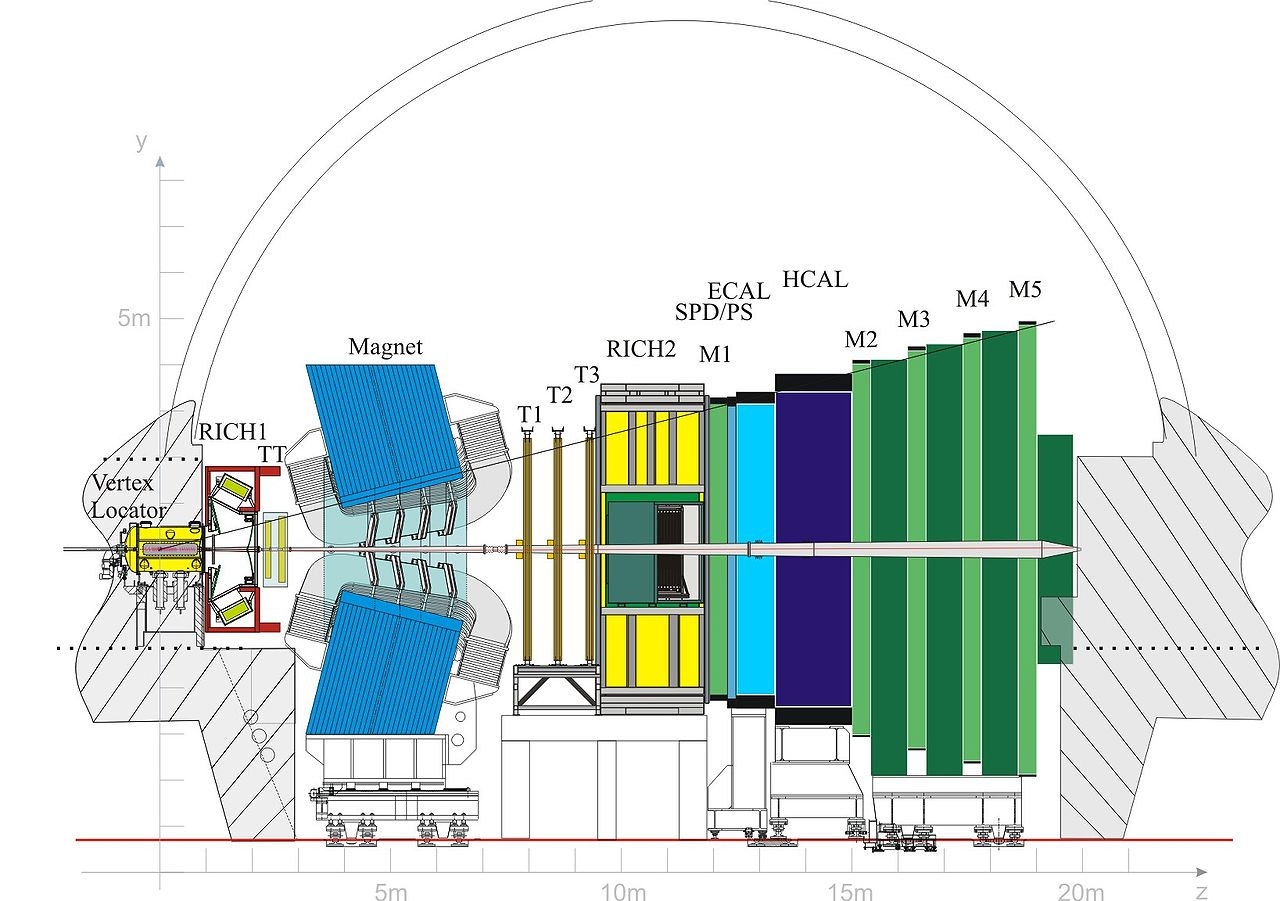
\includegraphics[scale=0.5]{LHCb_Det.jpg}
      \caption{The LHCb Detector along the bending plane.}
      \label{fig:LHCb_Collab}
    \end{figure}

    As B mesons are light (in comparision to other particles studied in the LHC), the decays products are produced at a shallow angle relivite the the beam pipe;
    this is the driving factor in the design of the exeperiment. 
    LHCb is a single arm forward spectormeter.
    Surrounding the point of collision is the \underline{Ve}rtex \underline{Lo}cator (VELO), this high precision detector uses silicon strips to detect ionising particles as they propogate from a collition and provides the coordinates of the particle in terms of R\footnote{Radial distance from the beam pipe.} and $\phi$\footnote{Asumthal angle.}.
    By reconstructing the paths of partics back to the intersection point, it can be identified wether or not the particular decay practicles are a product of the primary vertex\footnote{The position at which the protons collided.}, or a secondary vertex\footnote{The decay point of a short lived particle. i.e. B Meson.}.
    \par
    The Rich dectector, comprised of two subdectectors eitherside of the magnet, uses cherincov radiation to deduce the velocity of the particle. The silicon trackers, labeled TT and T1-3 in Figure~\ref{fig:LHCb_Collab}, calculate the angle deflection by the magnet. Be combining the velocity and angle of deflection, the mass, momentum and energy of the particles can be decuced from simple relitivistic kinematics.
    \par
    The meuon detectors, labeled M1-5 in Figure~\ref{fig:LHCb_Collab}, are important to detect muon's the detector. 
    This is of particular importance on LHCb as muons can be easily missidentified as charged pions, due to there simular mass and pions are a common decay product of the interects studied.
    \par
    HCAL and ECAL, shown in Figure~\ref{fig:LHCb_Collab}, are hadronic and electric calorimeters respectively. 
    Both measure the total energy of incomming particles.
    As the calorimeters are absorbing of the particles they detect, any leptonic particle reaching the M2-5 muon detectors can be assumed to be a muon.
    Electrons and Photons are absorbed by the ECAL and any Tauons would have decayed long before reaching the far muon detectors.

  \subsection{LHCb Upgrade} % (fold)
  \label{sub:lhcb_upgrade}

    With the advancments in accelerator technology, the detectors must also advance in order to make best use of the accelerators.
    The LHC is schedualed to increase its luminosity dureing \underline{L}ong \underline{S}hutdown \underline{2} (LS2), and as such LHCb will have to cope with this greater luminocity.
    The front end electronics of LHCb implement a hardware trigger and this is limited to a 1MHz maximum readout speed.
    Post LS2
    , LHCb will have to cope is a luminocity of $\mathcal{L} = 2.10^{33} cm^{-2}s^{-1}$, this is significatly greater than the current $\mathcal{L} = 4.10^{32} cm^{-2}s^{-1}$.
    A simple luminosity increase will not significantly increase that statistics for some statistical error dominated channels.
    To achieve this, greater resolution of the VELO and fully software triggers are required.
    Detailed in the \textit{`LHCb VELO Upgrade Technical Design Report'} \cite{velo_design_report} the main goals of the 2019 upgrade are as follows:

    \begin{easylist}[itemize]
      & Increase the luminosity to $\mathcal{L} = 2.10^{33} cm^{-2}s^{-1}$.
      & Read data from the detector at the bunch crossing frequancy, 40 Mhz.
      & Convert to a fully software bassed trigger.
    \end{easylist}

    % subsection lhcb_upgrade (end)

    \subsubsection{VELO Upgrade}

      Common with its predeseror, the upgraded VELO uses thin, retractable modules.
      The advange of this approuch is that during collisions, the modules can sit closer that otherwise possible to the beam line.
      The modules rectact for the beam fill, avoiding the radiation damage from the wider fill beams.
      In order to gain greater resolution of secondary verticies, the upgraded VELO will sit at $5.1$ mm from the beam at the closest pixel \cite{velo_design_report}.
      The current VELO achieves 8 mm \cite{velo_web}.
      
      \begin{figure}[ht]
        \centering
        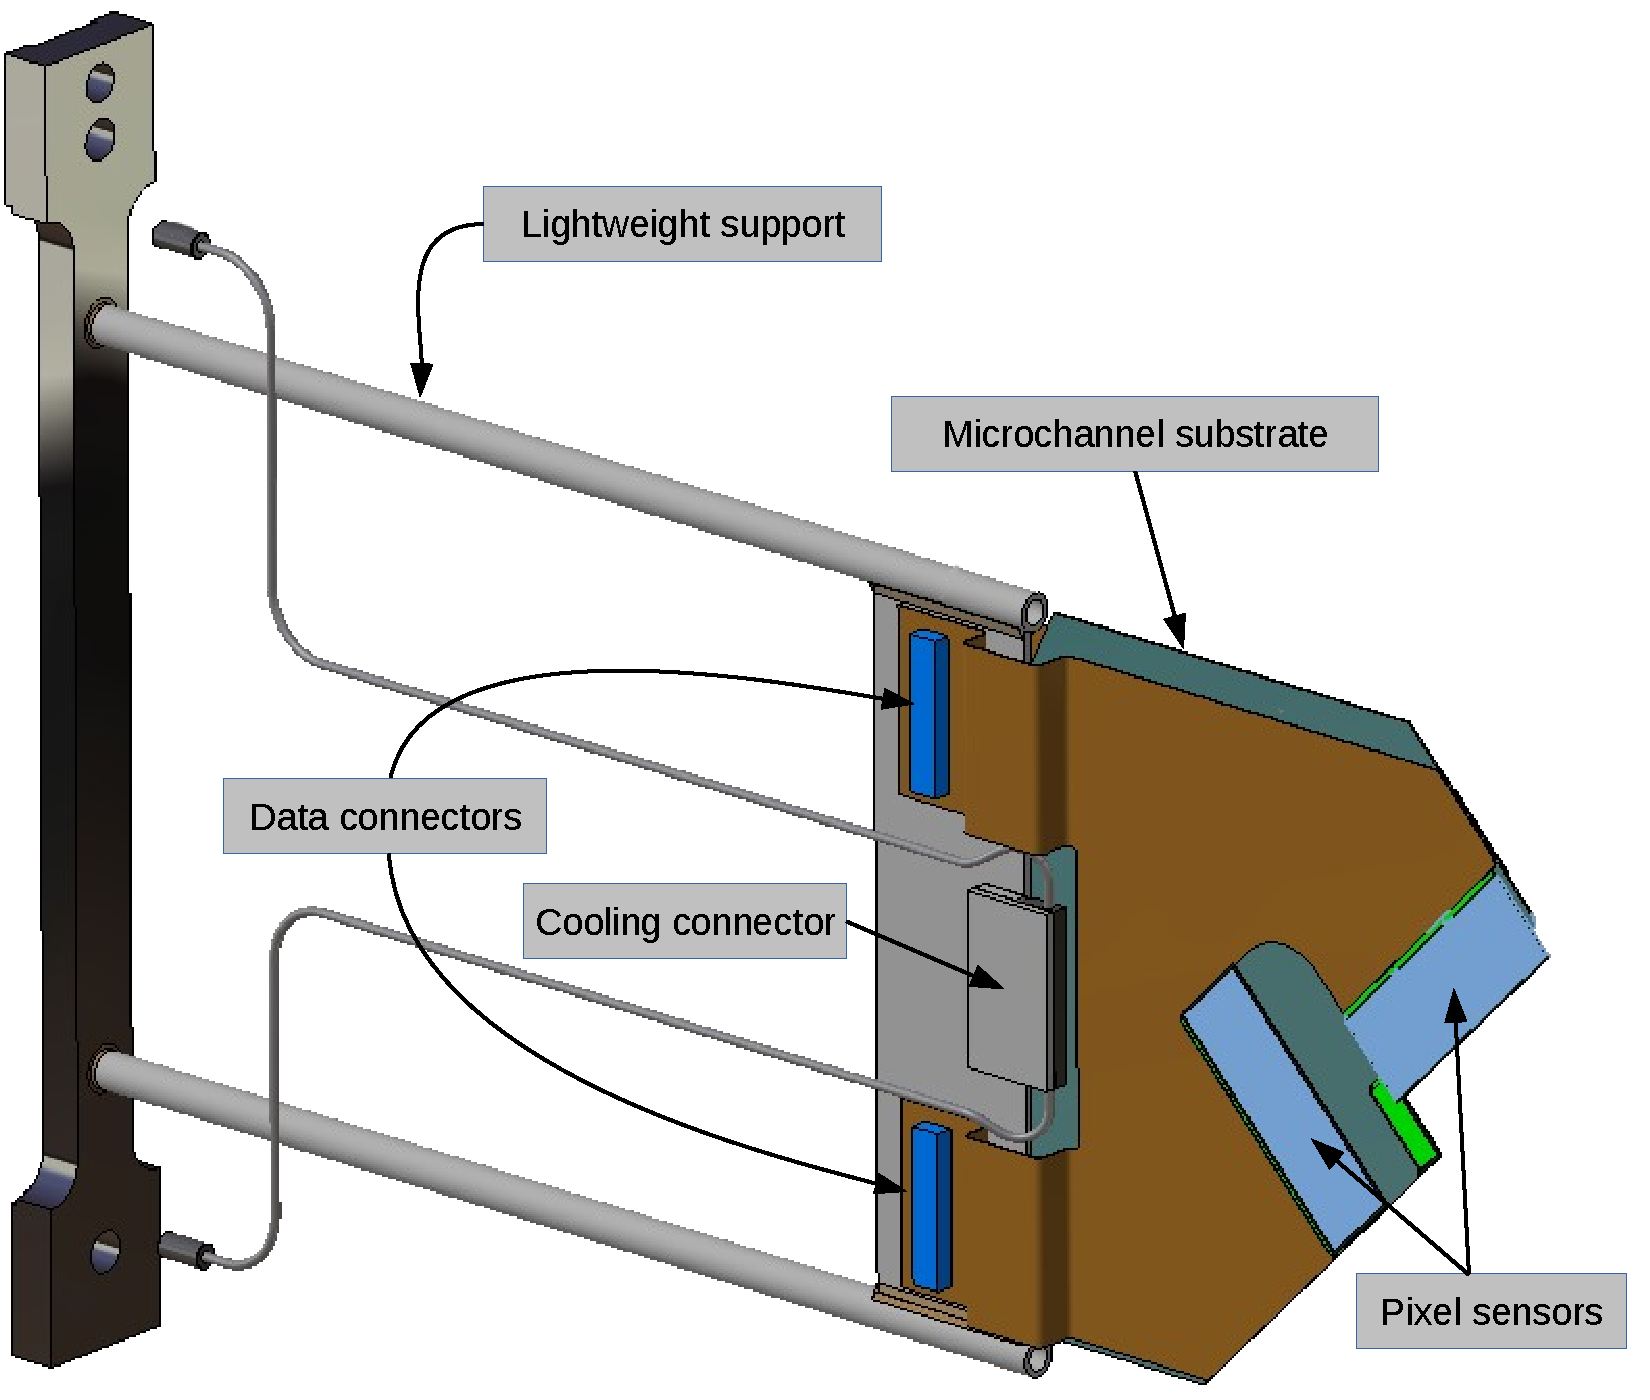
\includegraphics[width=0.75\textwidth]{module}
        \caption{The current module design. Two sensors are shown, the remaining two are mounted to the rear face of the module to for two horizontal rows - covering the right most area of the module (as viewed in the figure).}
        \label{fig:module}
      \end{figure}

      As previously mentioned, the current VELO uses silicon strips to detect particles.
      The upgraded VELO, however, will use silicon pixels.
      These pixels, $55 \mu m \times 55 \mu m$ in size and $200 \mu m$ thick \cite{velo_design_report}, are arranger in a 256 wide sqaure matrix on a ASIC chip.
      The pixels are arranged into groups of 8 to form a \underline{S}uper \underline{P}ixel (SP).
      The ASIC chips are arranged in a strait configeration of 3 and bonded to a sensor.
      Each module had 4 sersors, 2 a side, as shown in Figure~\ref{fig:module}. 
      The module is is cooled by bi-phase CO$^2$ in micro-channels etched into the microchannel substrate.
      \par
      The VELO modules will operate in the LHC secondary vacuum.
      It is seperated from the primary vacuum by RF foil that is 3.5mm from the beamline, at the closest point \cite{velo_design_report}.
      The foil is made of 250 $\mu m$ thick aluminum, it is required to be of this thickness to reduce the interacts with the collision decay products. 

      \subsubsection{Data Flow and Low Level Interface}   

      \underline{F}ield \underline{P}rogramable \underline{G}ate \underline{A}rrays (FPGAs) are extencively used in new technology due to there fast data transfer rates and revitility \cite{fpga}. 
      FPGAs are used in the \underline{D}ata \underline{Aq}uisition (DAQ) modules for speed and paralell procesing capabilities.
      The DAQ, in its simplest form, is a series of optical links, a data processing FPGA and a PCIe port for data transfer to the VELO computer system.
      \par
      The data from each SP is packaged in a 30 bit \underline{S}uper \underline{P}ixel \underline{P}acket (SPP). The SPP is comprised of  a (form most to least significant bits) 9 bit \underline{B}unch \underline{C}ross \underline{ID} (BCID); 13 bit SPP location information (horizontal and vertical coordinates); 8 bit SP hitmat.
      \par
      A GWT serialiser forms a 128 bit \textit{`frame'} comprising of a header (1010), four single bit parity flags and four SPPs.
      The parity flags indicate the parity of the four SPPs as a validation check for downstream processes.
      The data then is transmitted via an electrical to optical converter though optical fibers to the DAQ.
      \par
      In the DAQ is the \underline{L}ow \underline{L}evel \underline{I}nterface (LLI).
      The LLI is responcible for sorting the incomming data into time order and packaging the data in the correct form computer systems to optimise output bandwidth.
      Other processes included in the LLI are, descrabling and event isolation tagging.
      These processes will be discussed in more detail later in this document.



